\documentclass[letterpaper,11pt,oneside,reqno]{article}

%%%%%%%%%%%%%%%%%%%%%%%%%%%%%%%%%%%%%%%%%%%%%%%%%%%%%%%%%%%%

\usepackage[pdftex,backref=page,colorlinks=true,linkcolor=blue,citecolor=red]{hyperref}
\usepackage[alphabetic,nobysame]{amsrefs}

%%%%%%%%%%%%%%%%%%%%%%%%%%%%%%%%%%%%%%%%%%%%%%%%%%%%%%%%%%%%
%main packages
\usepackage{amsmath,amssymb,amsthm,amsfonts,mathtools}
\usepackage{graphicx,color}
\usepackage{upgreek}
\usepackage[mathscr]{euscript}

%equations
\allowdisplaybreaks
\numberwithin{equation}{section}

%tikz
\usepackage{tikz}
\usetikzlibrary{shapes,arrows,positioning,decorations.markings}

%conveniences
\usepackage{array}
\usepackage{adjustbox}
\usepackage{cleveref}
\usepackage{enumerate}
\usepackage{datetime}

%paper geometry
\usepackage[DIV=12]{typearea}

%%%%%%%%%%%%%%%%%%%%%%%%%%%%%%%%%%%%%%%%%%%%%%%%%%%%%%%%%%%%
%draft-specific
\synctex=1
% \usepackage{refcheck,comment}

%%%%%%%%%%%%%%%%%%%%%%%%%%%%%%%%%%%%%%%%%%%%%%%%%%%%%%%%%%%%
%this paper specific
\newcommand{\ssp}{\hspace{1pt}}

%%%%%%%%%%%%%%%%%%%%%%%%%%%%%%%%%%%%%%%%%%%%%%%%%%%%%%%%%%%%
\newtheorem{proposition}{Proposition}[section]
\newtheorem{lemma}[proposition]{Lemma}
\newtheorem{corollary}[proposition]{Corollary}
\newtheorem{theorem}[proposition]{Theorem}
%%%%%%%%%%%%%%%%%%%%%%%%%%%%%%%%%%%%%%%%%%%%%%%%%%%%%%%%%%%%
\theoremstyle{definition}
\newtheorem{definition}[proposition]{Definition}
\newtheorem{remark}[proposition]{Remark}
%%%%%%%%%%%%%%%%%%%%%%%%%%%%%%%%%%%%%%%%%%%%%%%%%%%%%%%%%%%%

\newenvironment{lnotes}{\section*{Notes for the lecturer}}{}

% \excludecomment{lnotes}

\begin{document}
\title{Lectures on Random Matrices
(Spring 2025)
\\Lecture 6: Double contour integral kernel. Steepest descent and local statistics}

\date{February 12, 2025\footnote{\href{https://lpetrov.cc/rmt25/}{\texttt{Course webpage}}
$\bullet$ \href{https://lpetrov.cc/simulations/model/random-matrices/}{\texttt{Live simulations}}
$\bullet$ \href{https://lpetrov.cc/rmt25/rmt25-notes/rmt2025-l06.tex}{\texttt{TeX Source}}
$\bullet$
Updated at \currenttime, \today}}

\author{Leonid Petrov}

\maketitle
\tableofcontents

\begin{lnotes}

\begin{itemize}
	\item GUE det structure

	\item Formulate Cauchy--Binet and Andreief

	\item Recall that $\rho_n=P_n$ and it is
	$\left( \det[\psi_i(x_j)]_{n\times n} \right)^2$, then reproduce the proofs here.

	\item Recall the Christoffel--Darboux formula:
	\begin{equation*}
		K_n(x,y)=\frac{e^{-\frac{x^2+y^2}{4}}}{\sqrt{2\pi}
		h_{n-1}}\,\frac{p_n(x)p_{n-1}(y)-p_{n-1}(x)p_n(y)}{x-y},
	\end{equation*}
	here $h_{n-1}=\sqrt{2\pi}(n-1)!$.
\end{itemize}

\end{lnotes}

\section{Recap: Determinantal structure of the GUE}

Last time, we proved the following result:
\begin{theorem}
\label{thm:determinantal_GUE}
The GUE correlation functions are given by
\[
\rho_k(x_1,\dots,x_k)=\det\Bigl[K_n(x_i,x_j)\Bigr]_{i,j=1}^k,
\]
with the correlation kernel
\[
K_n(x,y)=\sum_{j=0}^{n-1}\psi_j(x)\psi_j(y).
\]
Here
\begin{equation*}
	\psi_j(x)=\frac{1}{\sqrt{h_j}}\ssp p_j(x)\,e^{-x^2/4},
\end{equation*}
where \(p_j(x)\) are the monic Hermite polynomials, and \(h_j\) are the normalization constants so that
$\psi_j(x)$ are orthonormal in $L^2(\mathbb{R})$.
\end{theorem}

For this theorem, we need Cauchy--Binet summation formula
and Andreief identity (which is essentially the same as Cauchy--Binet, but when summation is
replaced by integration). Having these, we can write
\begin{align*}
	\rho_k(x_1,\dots,x_k)&=\frac{n!}{(n-k)!}\int_{\mathbb{R}^{n-k}} p(x_1,\dots,x_n) \,dx_{k+1}\cdots dx_n
	\\
	&=
	\frac{1}{(n-k)!\,\widehat{Z}_{n,2}}
	\sum_{\substack{\sigma,\tau\in S_n\\
	\sigma(k+1)=\tau(k+1),\ldots,\sigma(n)=\tau(n) }} \operatorname{sgn}(\sigma)\operatorname{sgn}(\tau)
	\prod_{i=1}^k \psi_{\sigma(i)-1}(x_i)\psi_{\tau(i)-1}(x_i)
	\\
	&=
	\mathrm{const}_n\sum_{I\subseteq [n],\,|I|=k}
	\sum_{\sigma',\tau'\in S(I)}
	\operatorname{sgn}(\sigma')\operatorname{sgn}(\tau')
	\prod_{i=1}^k \psi_{\sigma'(i)-1}(x_i)\psi_{\tau'(i)-1}(x_i)
	\\
	&=
	\mathrm{const}_n\sum_{I\subseteq [n],\,|I|=k}
	\det\left[ \psi_{i_\alpha}(x_j) \right]_{\alpha,j=1}^k
	\det\left[ \psi_{i_\alpha}(x_j) \right]_{\alpha,j=1}^k,
\end{align*}
where \(I=\{i_1,\ldots,i_k\}\) is a subset of \([n]\) of size \(k\), and \(S(I)\) is the set of permutations of \(I\).
The last sum of products of two determinants is
written by the Cauchy--Binet formula as
\begin{equation*}
	\mathrm{const}_n\cdot \det\left[ \sum_{j=0}^{n-1}\psi_j(x_\alpha)\psi_j(x_\beta) \right]_{\alpha,\beta=1}^k,
\end{equation*}
and finally the constant is equal to $1$ by Andreief identity.


%%%%%%%%%%%%%%%%%%%%%%%%%%%%%%%%%%%%%%%%%%%%%%%%%%%%%%%%%%%%
\section{Double Contour Integral Representation for the GUE Kernel}
\label{sec:double-contour}

\subsection{One contour integral representation for Hermite polynomials}

Recall that the GUE kernel is defined by
\[
K_N(x,y)=\sum_{n=0}^{N-1}\psi_n(x)\psi_n(y),
\]
with the orthonormal functions
\[
\psi_n(x)=\frac{1}{\sqrt{h_n}}\,p_n(x)\,e^{-x^2/4},
\]
where the (monic, probabilists') Hermite polynomials are given by
\begin{equation}
\label{eq:hermite_def}
	p_n(x)=(-1)^n e^{x^2/2}\frac{d^n}{dx^n}\,e^{-x^2/2}.
\end{equation}
Note that the monic Hermite polynomials are uniquely defined by the
orthogonality property. We are not proving \eqref{eq:hermite_def} here,
it is an exercise.
\begin{lemma}[Generator function for Hermite polynomials]
	\label{lem:hermite_gen}
	We have
	\[
		\exp\Bigl(xt-\frac{t^2}{2}\Bigr)=\sum_{n\ge0}p_n(x)\frac{t^n}{n!}.
	\]
	The series converges for all \(t\) since the left-hand side is an entire function of \(t\).
\end{lemma}
\begin{proof}
Write the generating function as
\[
	\sum_{n\ge0}p_n(x)\frac{t^n}{n!}
	=\sum_{n\ge0}\frac{(-1)^n t^n}{n!}\,e^{x^2/2}\frac{d^n}{dx^n}\,e^{-x^2/2}.
\]
Since the factor \(e^{x^2/2}\) does not depend on \(n\), we can factor it out:
\[
	\sum_{n\ge0}p_n(x)\frac{t^n}{n!}= e^{x^2/2}\sum_{n\ge0}\frac{(-t)^n}{n!}\frac{d^n}{dx^n}\,e^{-x^2/2}.
\]
Now, recall Taylor's theorem: for any holomorphic function \(f\) we have
\[
	f(x-t)=\sum_{n\ge0}\frac{(-t)^n}{n!}f^{(n)}(x).
\]
Applying this with \(f(x)=e^{-x^2/2}\), we deduce that
\[
	\sum_{n\ge0}\frac{(-t)^n}{n!}\frac{d^n}{dx^n}\,e^{-x^2/2}= e^{-(x-t)^2/2}.
\]
Thus, our generating function becomes
\[
	\sum_{n\ge0}p_n(x)\frac{t^n}{n!} = e^{x^2/2}\, e^{-(x-t)^2/2},
\]
as desired.
\end{proof}


By Cauchy's integral formula we can write using \Cref{lem:hermite_gen}:
\begin{equation}
\label{eq:pn-formula}
p_n(x)=\frac{n!}{2\pi i}\oint_C\frac{\exp\Bigl(xt-\frac{t^2}{2}\Bigr)}{t^{n+1}}\,dt,
\end{equation}
where the contour \(C\) is a simple closed curve encircling the origin.
Indeed, here we use the complex analysis property
\begin{equation*}
	\frac{1}{2\pi i}\oint_C \frac{1}{z^{k+1}}\ssp dz=\begin{cases}
		1,&\text{ if }k=0,\\
		0,&\text{ if }k\neq0,
	\end{cases}
\end{equation*}
so \eqref{eq:pn-formula} is simply a complex analysis version of the
operation of extracting the coefficient of \(t^n\) in the Taylor expansion.

Therefore,
\begin{equation*}
	\psi_n(x)=\frac{1}{\sqrt{h_n}}\,p_n(x)\,e^{-x^2/4}=
	\frac{e^{-x^2/4}}{\sqrt{h_n}}\frac{n!}{2\pi i}\oint_C\frac{\exp\Bigl(xt-\frac{t^2}{2}\Bigr)}{t^{n+1}}\,dt.
\end{equation*}

\subsection{Another contour integral representation for Hermite polynomials}

We start with the Fourier transform identity
\[
\int_{-\infty}^{\infty} \exp\Bigl(-\frac{t^2}{2} + i\,t\,x\Bigr)\,dt
=\sqrt{2\pi}\,e^{-x^2/2}.
\]
Differentiating both sides \(n\) times with respect to \(x\) yields
\[
\frac{d^n}{dx^n}\Bigl(e^{-x^2/2}\Bigr)
=\frac{1}{\sqrt{2\pi}}\int_{-\infty}^{\infty} (i\,t)^n\,e^{-t^2/2+ i\,t\,x}\,dt.
\]
Recalling the definition
\[
p_n(x)=(-1)^n\,e^{x^2/2}\,\frac{d^n}{dx^n}\Bigl(e^{-x^2/2}\Bigr),
\]
we obtain
\[
p_n(x)=\frac{(-1)^n\,e^{x^2/2}}{\sqrt{2\pi}}\int_{-\infty}^{\infty}(i\,t)^n\,e^{-t^2/2+ i\,t\,x}\,dt.
\]

Next, perform the change of variable
\[
s=i\,t,\quad\text{so that}\quad t=-i\,s,\quad dt=-i\,ds.
\]
Under this substitution the factors transform as follows:
\[
(i\,t)^n = s^n,
\]
and the exponent becomes
\[
-\frac{t^2}{2}+ i\,t\,x
= -\frac{(-i\,s)^2}{2}+ i\,(-i\,s)\,x
= \frac{s^2}{2}+ s\,x.
\]
Thus, the integral transforms into
\[
\int_{-\infty}^{\infty}(i\,t)^n\,e^{-t^2/2+ i\,t\,x}\,dt
= -i \int_{-i\infty}^{i\infty} s^n\,e^{s^2/2+ s\,x}\,ds.
\]
Substituting back we have
\[
p_n(x)=\frac{(-1)^n\,e^{x^2/2}}{\sqrt{2\pi}}\;(-i)
\int_{-i\infty}^{i\infty} s^n\,e^{s^2/2+ s\,x}\,ds.
\]
That is,
\[
p_n(x)=\frac{i\,(-1)^{n+1}\,e^{x^2/2}}{\sqrt{2\pi}}
\int_{-i\infty}^{i\infty} s^n\,e^{s^2/2+ s\,x}\,ds.
\]
Finally, change the sign of $s$, and we get:
\[
p_n(x)=\frac{i\,e^{x^2/2}}{\sqrt{2\pi}}
\int_{-i\infty}^{i\infty} s^n\,e^{s^2/2- s\,x}\,ds.
\]
Therefore,
\[
\psi_n(x)=\frac{i\,e^{x^2/4}}{\sqrt{2\pi\,h_n}}
\int_{-i\infty}^{i\infty} s^n\,e^{s^2/2- s\,x}\,ds.
\]

\subsection{Normalization of Hermite polynomials}

\begin{lemma}
	\label{lem:hermite_norm}
	We have
	\begin{equation*}
		h_n=\int_{-\infty}^{\infty} p_n(x)^2\,e^{-x^2/2}\,dx=n!\sqrt{2\pi}.
	\end{equation*}
\end{lemma}
\begin{proof}
Multiply the generating function
\[
	\exp\Bigl(xt-\frac{t^2}{2}\Bigr)=\sum_{n\ge0}p_n(x)\frac{t^n}{n!}
\]
with a second copy (with parameter \(s\)):
\[
	\exp\Bigl(xs-\frac{s^2}{2}\Bigr)=\sum_{m\ge0}p_m(x)\frac{s^m}{m!}.
\]
Then,
\[
	\exp\Bigl(xt-\frac{t^2}{2}\Bigr)\exp\Bigl(xs-\frac{s^2}{2}\Bigr)
	=\sum_{n,m\ge0}p_n(x)p_m(x)\frac{t^n s^m}{n!m!}.
\]
Integrate both sides against \(e^{-x^2/2}\,dx\). Using the orthogonality
\[
	\int_{-\infty}^{\infty}p_n(x)p_m(x)e^{-x^2/2}dx=h_n\delta_{nm},
\]
the right-hand side becomes
\[
	\sum_{n\ge0}\frac{h_n}{(n!)^2}(ts)^n.
\]
On the left-hand side, we have
\[
	\int_{-\infty}^{\infty}e^{-x^2/2}\exp\Bigl(x(t+s)-\frac{t^2+s^2}{2}\Bigr)dx.
\]
Completing the square in \(x\) or recalling the standard Gaussian integral yields
\[
	\sqrt{2\pi}\exp\Bigl(\frac{(t+s)^2-(t^2+s^2)}{2}\Bigr)
	=\sqrt{2\pi}\exp(ts).
\]
Thus, we obtain
\[
	\sqrt{2\pi}\exp(ts)=\sum_{n\ge0}\frac{h_n}{(n!)^2}(ts)^n.
\]
Expanding the left side as
\[
	\sqrt{2\pi}\sum_{n\ge0}\frac{(ts)^n}{n!},
\]
and comparing coefficients, we conclude that
\[
	\frac{h_n}{(n!)^2}=\frac{\sqrt{2\pi}}{n!}\quad\Longrightarrow\quad h_n=n!\sqrt{2\pi}.
\]
This completes the proof.
\end{proof}

\subsection{Double contour integral representation for the GUE kernel}

We can sum up the kernel (essentially, this is
another proof of the Christoffel--Darboux formula):
\begin{equation}\begin{split}
	K_n(x,y)&=
	\sum_{k=0}^{n-1}\psi_k(x)\psi_k(y)
	\\&=
	\frac{e^{\frac{x^2-y^2}{4}}}{(2\pi)^2}
	\oint_C dt\int_{-i\infty}^{i\infty}ds\ssp
	\exp\left\{ -\frac{t^2}{2}+xt+\frac{s^2}{2}-ys \right\}
	\underbrace{\sum_{k=0}^{n-1}
	s^k t^{-k-1}}_{\frac{1-(s/t)^n}{t-s}}.
\end{split}\label{eq:K_n_sum}\end{equation}
Here we used the two contour integral representations for Hermite polynomials,
and the explicit norm (\Cref{lem:hermite_norm}).
At this point, the $t$ contour is a small circle around $0$, and
the $s$ contour is a vertical line in the complex plane.
Their mutual position can be arbitrary at this point --- the $s$ contour
goes along the imaginary line.
Indeed, the fraction
$\frac{1-(s/t)^n}{t-s}$ does not have a singularity at $s=t$ due to the
cancellation.

Let us now move the $s$ contour to be to the left of the $t$ contour,
as in \Cref{fig:contours}.
On the new contours, we have $|s|>|t|$.
Now we can add the summands $s^k t^{-k-1}$
for all $k\le -1$
into the sum in
\eqref{eq:K_n_sum}.
Indeed, for $|s|>|t|$, the series in $k$ converges, while the
summand $s^kt^{-k-1}$ has zero residue at $0$ and thus adding the
summands does not change the value of the integral.

\begin{figure}[htpb]
	\centering
	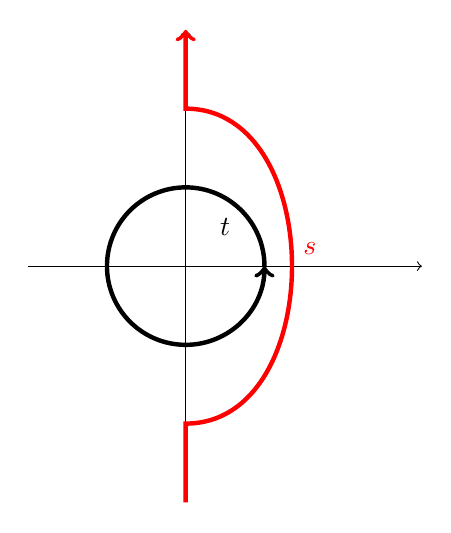
\begin{tikzpicture}[scale=1]
		% Draw coordinate axes
		\draw[->] (-2,0) -- (3,0);
		\draw[->] (0,-3) -- (0,3);

		% t contour: unit circle, counterclockwise
		\draw[ultra thick,->] (1,0) arc (0:360:1);
		% Place the t label near the contour (at 45° outside the circle)
		\coordinate (TLabel) at (.5,.5);
		\node at (TLabel) {\(t\)};

		% s contour: vertical line (imaginary axis) with a detour near the origin
		% It starts at (0,-3), goes vertically to (0,-2), then detours to (0,2)
		% via a Bézier curve (pushed to the right), and finally resumes vertically to (0,3).
		\draw[ultra thick,->,red]
			(0,-3)
			-- (0,-2)
			.. controls (1.8,-2) and (1.8,2) .. node[midway, above right] {\(s\)} (0,2)
			-- (0,3);
	\end{tikzpicture}
	\caption{Integration contours for the GUE kernel \eqref{eq:K_n_GUE_kernel}.}
	\label{fig:contours}
\end{figure}

With this extension of the sum, formula \eqref{eq:K_n_sum} becomes
\begin{equation}
	\label{eq:K_n_GUE_kernel}
	K_n(x,y)=\frac{e^{(y^2-x^2)/4}}{(2\pi)^2}
	\oint_C dt\int_{-i\infty}^{i\infty}ds\ssp
	\frac{\exp\left\{ \frac{s^2}{2}-sy-\frac{t^2}{2}+tx \right\}}{s-t}\left( \frac{s}{t} \right)^n
	.
\end{equation}

\begin{remark}
	The $s$ contour passes to the right of the $t$ contour, but it might as well
	pass to the left of it. Indeed, one can deform the $s$ contour to the left
	while picking the residue at $s=t$:
	\begin{equation*}
		\operatorname{Res}\limits_{s=t}
		\frac{\exp\left\{ \frac{s^2}{2}-sy-\frac{t^2}{2}+tx \right\}}{s-t}\left( \frac{s}{t} \right)^n
		=-e^{t(x-y)}.
	\end{equation*}
	This function is entire in $t$, and its
	integral over the $t$ contour is zero.
	Therefore, there is no difference where the $s$ contour passes with respect to the $t$ contour.
\end{remark}


\subsection{Extensions}

Many other versions of the GUE / unitary invariant ensembles admit determinantal structure:
\begin{enumerate}
	\item The GUE corners process \cite{johansson2006eigenvalues}
    \item The Dyson Brownian motion (e.g., add a GUE to a diagonal matrix)
			\cite{nagao1998multilevel}
		\item GUE corners plus a fixed matrix \cite{Ferrari2014PerturbedGUE}
    \item Corners invariant ensembles with fixed eigenvalues $UDU^\dagger$, where $D$ is a fixed diagonal matrix and $U$ is Haar distributed
			on the unitary group \cite{Metcalfe2011GT}
	\end{enumerate}

We will discuss the corners process structure
in the next
\href{https://lpetrov.cc/rmt25/rmt25-notes/rmt2025-l07.pdf}{Lecture 7}.

%%%%%%%%%%%%%%%%%%%%%%%%%%%%%%%%%%%%%%%%%%%%%%%%%%%%%%%%%%%%

%%%%%%%%%%%%%%%%%%%%%%%%%%%%%%%%%%%%%%%%%%%%%%%%%%%%%%%%%%%%
\section{Steepest descent --- generalities for single integrals}
%%%%%%%%%%%%%%%%%%%%%%%%%%%%%%%%%%%%%%%%%%%%%%%%%%%%%%%%%%%%

\subsection{Setup}

In many problems arising in random matrix theory—as well as in asymptotic analysis more generally—it is necessary to evaluate integrals of the form
\begin{equation}
	\label{eq:general-integral}
	I(\Lambda)=\int_{\gamma} e^{\Lambda f(z)}\ssp \phi(z)\,dz,
\end{equation}
where
\begin{itemize}
	\item $\Lambda>0$ is a large parameter,
	\item $f(z)$ and $\phi(z)$ are holomorphic functions in a neighborhood of the contour $\gamma\subset\mathbb{C}$,
	\item and the contour $\gamma$ is chosen in such a way that the integral converges.
\end{itemize}
The \emph{method of steepest descent} (also known as the \emph{saddle point method}) provides a systematic procedure for obtaining the asymptotic behavior of $I(\Lambda)$ as $\Lambda\to+\infty$.

The key observation is that for large $\Lambda$, the
exponential term $e^{\Lambda f(z)}$ is highly oscillatory or
decaying, so that the main contributions to the integral
come from small neighborhoods of points where the real part
of $f(z)$ is maximal.
Moreover, since we can deform the integration contour $\gamma$
to pick points where $\operatorname{Re}f(z)$ is even bigger, it makes sense to find
points \emph{not only on the original contour}
where $\operatorname{Re}f(z)$ is maximal.
Such \emph{critical} (or \emph{saddle}) points are
found from the equation with the complex derivative:
\begin{equation*}
	f'(z)=0
\end{equation*}
Indeed, since $\operatorname{Re}f(z)$
is harmonic and $f(z)$ satisfies the Cauchy--Riemann equations,
the condition $f'(z)=0$ is equivalent to the condition that $\operatorname{Re}f(z)$
has zero gradient. Moreover, by harmonicity, all critical points of
$\operatorname{Re}f(z)$ are saddle-like.

Once the saddle points are identified, one deforms the
contour $\gamma$ to $\Gamma$ so that $\Gamma$ passes
through the saddle point(s)
with the maximal value of $\operatorname{Re}f(z)$, and, moreover,
such that on the rest of the new contour $\Gamma$ the
real part of $f(z)$ is strictly less than the value(s) at the saddle point(s).
The decrease of $\operatorname{Re}f(z)$ along $\Gamma$ may be ensured
if one picks $\Gamma$ to be \emph{steepest descent} for $\operatorname{Re}f(z)$.
By holomorphicity of $f(z)$, the steepest descent
of $\operatorname{Re}$ is equivalent to the condition that
the imaginary part of $f(z)$ is constant along $\Gamma$.

\begin{remark}
	\label{rem:steepest-descent}
	In practical applications, one does not
	need $\Gamma$ to be fully steepest descent (it is usually hard to control).
	One can either choose $\Gamma$ to be steepest descent
	in a neighborhood of the critical point and estimate the real part outside,
	or simply estimate the change of $\operatorname{Re}f(z)$ directly along a given contour.
\end{remark}

\begin{remark}
	\label{rem:residues}
	The function $\phi(z)$ might not be holomorphic, and might have poles. The
	deformation of the contour from $\gamma$ to $\Gamma$ might pick residues
	at these poles. These residues can be harmless (easy to account for) or
	not (hard to account for; or affect the asymptotics of the integral),
	and one has to be careful with the contour deformation.
\end{remark}

Despite the caveats in \Cref{rem:steepest-descent,rem:residues},
in what follows in this section we will discuss the
easiest case of steepest descent analysis.
We also assume that there is only one saddle point $z_0$
to take care of.

%%%%%%%%%%%%%%%%%%%%%%%%%%%%%%%%%%%%%%%%%%%%%%%%%%%%%%%%%%%%
\subsection{Saddle points and steepest descent paths}
%%%%%%%%%%%%%%%%%%%%%%%%%%%%%%%%%%%%%%%%%%%%%%%%%%%%%%%%%%%%

\begin{definition}[Saddle point]
	A point $z_0\in\mathbb{C}$ is called a \emph{saddle point} of $f(z)$ if
	\[
		f'(z_0)=0.
	\]
	We shall assume in what follows that at every saddle point under consideration the second derivative satisfies
	\[
		f''(z_0)\neq 0.
	\]
\end{definition}

\begin{definition}[Steepest descent path]
	Let $z_0$ be a saddle point of $f(z)$. A curve $\Gamma\subset\mathbb{C}$ passing through $z_0$ is called a \emph{steepest descent path} for $f(z)$ if along $\Gamma$ the imaginary part of $f(z)$ is constant (i.e.,
	\(
		\operatorname{Im}\bigl(f(z)\bigr)=\operatorname{Im}\bigl(f(z_0)\bigr)
	\)
	for all $z\in\Gamma$), which implies that the real part
	$\operatorname{Re}\bigl(f(z)\bigr)$ decreases away from
	$z_0$.
\end{definition}

In a neighborhood of a saddle point $z_0$,
\[
	z=z_0+w,
	\qquad 
	f(z)=f(z_0)+\frac{1}{2}f''(z_0)w^2 + O(w^3).
\]
If we denote
\[
	f''(z_0)=|f''(z_0)|e^{i\theta_0},
\]
then writing $w=r\,e^{i\varphi}$, we obtain
\[
	f(z)=f(z_0)+\frac{1}{2}|f''(z_0)|r^2e^{i(2\varphi+\theta_0)}+O(r^3).
\]
For the imaginary part to remain constant in a neighborhood
of $z_0$, and, moreover,
for the phase of the quadratic term to be $\pi$ modulo $2\pi$, one must choose $\varphi$ so that
\begin{equation}
	\label{eq:steepest-descent-direction}
	2\varphi+\theta_0=\pi \quad (\operatorname{mod}\,2\pi).
\end{equation}
We need the phase $\pi$ so that the exponent is negative, for the integral to converge.

There are two directions satisfying \eqref{eq:steepest-descent-direction}
through $z_0$, and we use both of them for our contour $\Gamma$.
Along these directions, one finds that
\[
	\operatorname{Re}\bigl(f(z)\bigr)=\operatorname{Re}\bigl(f(z_0)\bigr)-\frac{1}{2}|f''(z_0)|r^2+O(r^3),
\]
so that $\operatorname{Re}(f(z))$ is maximal at $z=z_0$ and decays quadratically as one moves away from $z_0$ along the steepest descent paths.

%%%%%%%%%%%%%%%%%%%%%%%%%%%%%%%%%%%%%%%%%%%%%%%%%%%%%%%%%%%%
\subsection{Local asymptotic evaluation near a saddle point}
%%%%%%%%%%%%%%%%%%%%%%%%%%%%%%%%%%%%%%%%%%%%%%%%%%%%%%%%%%%%

Assume now that the contour $\gamma$ in \eqref{eq:general-integral} has been deformed so that it passes through a saddle point $z_0$ along a steepest descent path. In a small neighborhood of $z_0$, we write
\[
	z=z_0+w,
\]
so the local contribution of a neighborhood of $z_0$ to the integral is
\begin{equation}
	\label{eq:local-contribution}
	I_{z_0}(\Lambda)=e^{\Lambda f(z_0)}\phi(z_0)
	\int_{-\infty}^{\infty} e^{\Lambda\frac{1}{2}f''(z_0)w^2}\,dw
	\Bigl(1+O\Bigl(\frac{1}{\Lambda}\Bigr)\Bigr).
\end{equation}
Here the integration is taken along the steepest descent direction, so that the quadratic term in the exponent is real and negative. (That is, by the choice \eqref{eq:steepest-descent-direction}, we have $\operatorname{Re}\bigl(f''(z_0)w^2\bigr)=-|f''(z_0)|r^2$.) Then the Gaussian integral evaluates to
\[
	\int_{-\infty}^{\infty} e^{-\Lambda\frac{|f''(z_0)|}{2}r^2}\,dr
	=\sqrt{\frac{2\pi}{\Lambda |f''(z_0)|}}.
\]
Hence, we
arrive at the following fundamental result.

\begin{theorem}[Local asymptotics via steepest descent]
	\label{thm:steepest-descent}
	Let $z_0$ be a saddle point of $f(z)$ with $f'(z_0)=0$ and $f''(z_0)\neq 0$, and assume that $\phi(z)$ is holomorphic in a neighborhood of $z_0$. Then, as $\Lambda\to+\infty$, the contribution of a small neighborhood of $z_0$ to the integral \eqref{eq:general-integral} is given by
	\begin{equation}
		\label{eq:local-asymptotics}
		I_{z_0}(\Lambda)
		\sim e^{\Lambda f(z_0)}\ssp \phi(z_0)
		\sqrt{\frac{2\pi}{\Lambda\,|f''(z_0)|}},\qquad \Lambda\to+\infty.
	\end{equation}
	Moreover, the behavior \eqref{eq:local-asymptotics}
	captures the full asymptotic behavior of the 
	integral \eqref{eq:general-integral} 
	as long as on the new contour $\Gamma$,
	the real part of $f(z)$ is maximized at $z_0$ and is separated
	from $\operatorname{Re}f(z_0)$ everywhere else on $\Gamma$ outside of a 
	small neighborhood of $z_0$.
\end{theorem}

Under appropriate assumptions (typically, if $f$ and $\phi$ are holomorphic on a neighborhood that can be reached by the deformed contour and if the contributions away from the saddle points are exponentially small), one may show that the error in approximating the full integral by the sum of the local contributions is itself exponentially small relative to the leading order terms. In many cases, the next-order corrections can be computed by carrying the expansion in \eqref{eq:local-contribution} to higher order in $w$. (See, e.g., \cite{olver1974asymptotics} for a systematic treatment.)

%%%%%%%%%%%%%%%%%%%%%%%%%%%%%%%%%%%%%%%%%%%%%%%%%%%%%%%%%%%%




















\appendix
\setcounter{section}{5}

\section{Problems (due 2025-03-12)}





\bibliographystyle{alpha}
\bibliography{bib}


\medskip

\textsc{L. Petrov, University of Virginia, Department of Mathematics, 141 Cabell Drive, Kerchof Hall, P.O. Box 400137, Charlottesville, VA 22904, USA}

E-mail: \texttt{lenia.petrov@gmail.com}


\end{document}
